\documentclass[12pt]{article}
\usepackage[svgnames,x11names,table]{xcolor}
\usepackage{hyperref}
\usepackage{graphicx}
\usepackage{parskip}
\usepackage{float}
\usepackage{amsmath}
\usepackage{amssymb}
\usepackage{enumitem}
\usepackage[thicklines]{cancel}

\hypersetup{
    colorlinks,
    citecolor=black,
    filecolor=black,
    linkcolor=RoyalBlue4,
    urlcolor=RoyalBlue4,
}

\title{PEU 453 Assignment 2}
\author{Mohamed Hussien El-Deeb (201900052)}
\date{}

\begin{document}

\maketitle
\tableofcontents

\section{Problem 2.4}

\begin{figure}[H]
    \centering
    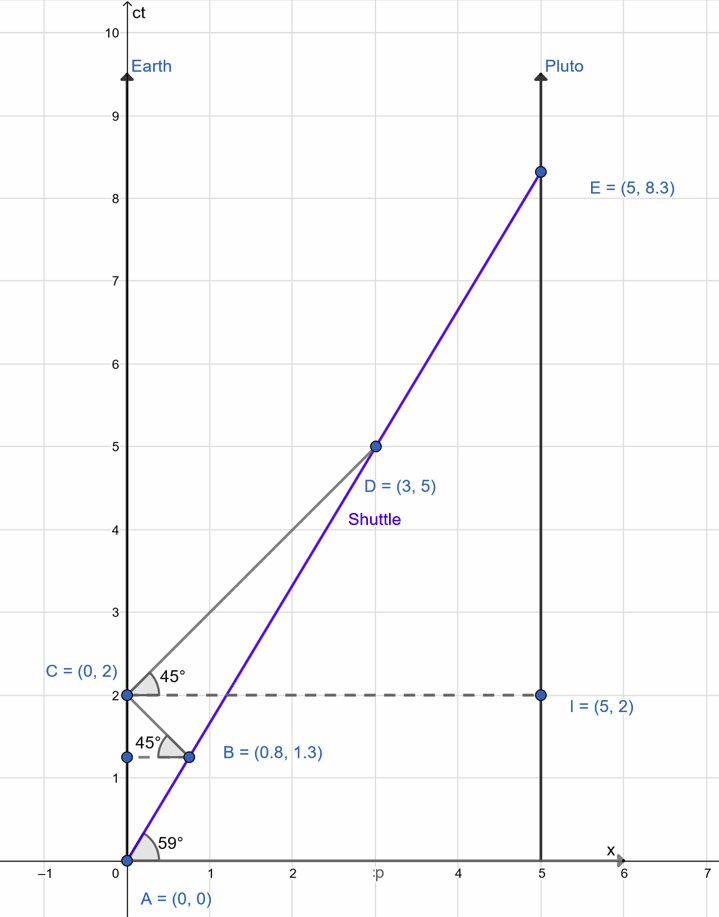
\includegraphics[scale=0.4]{Q1A.png}
\end{figure}

\renewcommand{\labelenumi}{\alph{enumi}.}
\begin{enumerate}
    \item The boss expects to have the message arrive at 2 Tm however as he is traveling 0.6C it should arrive after \(\Delta t'= \gamma \Delta t = 1\text{Tm} \frac{1}{\sqrt{1-0.6^2}} = 1.25\text{Tm} \) which is 2.5Tm in proper time from the start of the journey. It arrives at approximately 5.
    \item The light message takes time to travel and the distance it requires to travel means that it needs to spends more time than the nap duration.
    \item is the \(T_B = 1.25Tm,\, T_D = 5Tm,\, \Delta t = T_D - T_B = 3.75Tm,\, \Delta T' = \frac{\Delta T}{\gamma} = 0.8 * 3.75Tm = 3Tm \)
    \item
\end{enumerate}

\begin{figure}[H]
    \centering
    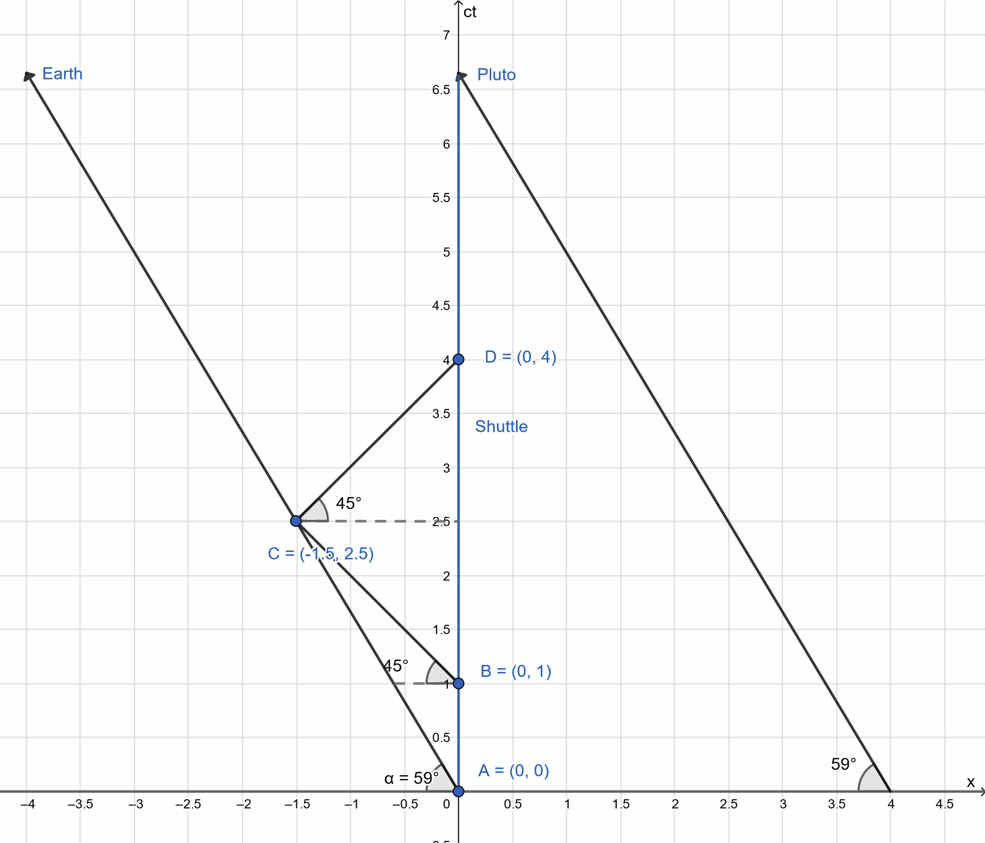
\includegraphics[scale=0.4]{Q1D.png}
\end{figure}

\newpage

\section{Problem 2.6}

\begin{enumerate}
    \item Since the both events happen at the same location in the station frame \(\Delta T' = \frac{\Delta T}{\gamma} = \sqrt{1-\beta^2} 100 = 80m \)
    \item They are equal since the the event A and B mark the beginning and the end of the train touching the train station.
\end{enumerate}

\newpage

\section{Problem 2.9}

\begin{enumerate}
    \item For A:

          \(v=\frac{d}{t} = \frac{6}{13}\quad \Delta T' = \frac{\Delta T}{\gamma} = 13Tm\sqrt{1-\frac{36}{169}} = \sqrt{133} \approx 11.5 \)

    \item For B:

          \(v=\frac{d}{t} = \frac{3\pi}{13}\quad \Delta T' = 13Tm\sqrt{1-{\frac{3\pi}{13}}^2} = \sqrt{133} \approx 9 \)
\end{enumerate}

\newpage

\section{Problem 2.10}

\[L - vt_1 = ct_1 \implies t_1 = \frac{L}{c + v}\]
\[L + vt_2 = ct_2 \implies t_2 = \frac{L}{c - v}\]
\[t = t_1 + t_2 = \frac{L}{c + v} + \frac{L}{c - v} = \frac{2L}{c}\frac{1}{1-{(\frac{v}{c})}^2} = \frac{2L}{c} \gamma^2\]


\[
    t' = \frac{2L'}{c}
\]

Where \(L' = L \gamma\quad\&\quad\gamma = \frac{1}{\sqrt{1-{(\frac{v}{c})}^2}}\)

\[
    t = t' \gamma
\]

\newpage

\section{Problem 2.11}

\begin{figure}[H]
    \centering
    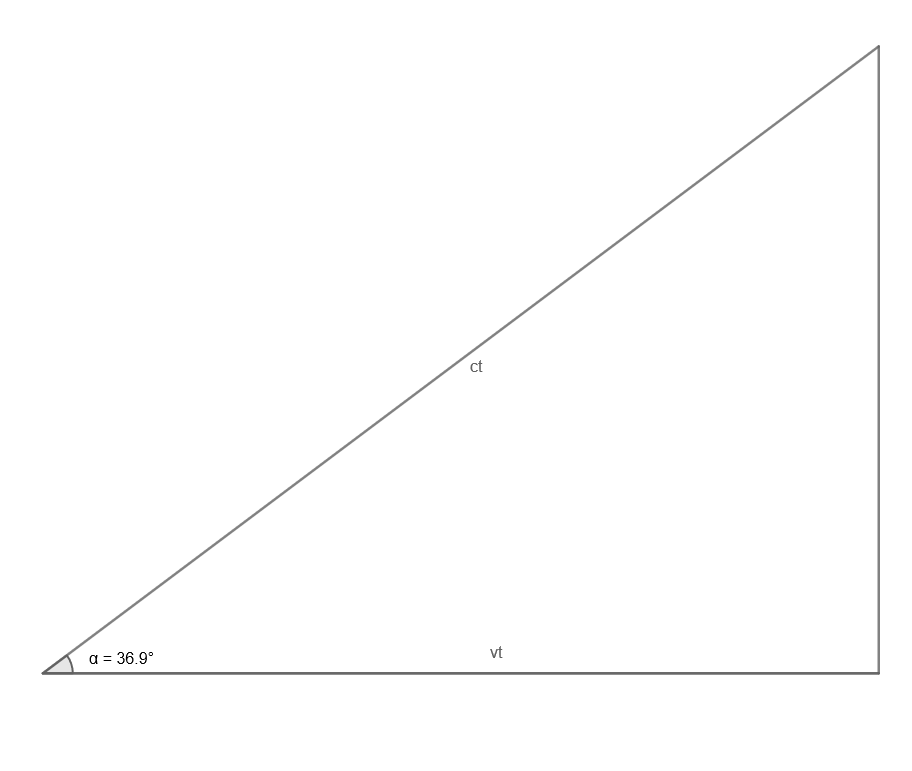
\includegraphics[scale=0.4]{Q5.png}
\end{figure}

\(\theta = \cos^-1(\frac{4}{5}) = 36.87\)

\newpage

\bibliographystyle{plain}
\bibliography{references}
\nocite{El-Deeb_PEU-453_Assignments}

\end{document}